\appendix

% \renewcommand{\chaptermark}[1]{%
% \markboth{\thechapter.%
% \ \chaptername.\ #1}{}}

\chapter{A lineáris megoldó program kódja}\label{chap: függ linprog}


 \lstinputlisting{"MATLAB/linear_system/main.m"}
 \lstinputlisting{"MATLAB/linear_system/init_system.m"}
  \lstinputlisting{"MATLAB/linear_system/integration_parameters.m"}
  \lstinputlisting{"MATLAB/linear_system/init_conditions.m"}
 \lstinputlisting{"MATLAB/linear_system/timestep.m"}
 

\chapter{A nemlineáris megoldó program kódja}\label{chap: függ nemlinprog}

\lstinputlisting{"MATLAB/nonlinear_system/main.m"}
 \lstinputlisting{"MATLAB/nonlinear_system/init_system.m"}
 \lstinputlisting{"MATLAB/nonlinear_system/integration_parameters.m"}
 \lstinputlisting{"MATLAB/nonlinear_system/init_conditions.m"}
 \lstinputlisting{"MATLAB/nonlinear_system/timestep.m"}
 \lstinputlisting{"MATLAB/nonlinear_system/resisting_force.m"}
 \lstinputlisting{"MATLAB/nonlinear_system/tangent_stiffness.m"}

\chapter{A lineáris megoldó program eredményei}\label{chap: függ eredmények}

\section{A \ref{subsec:lingerj} gerjesztett rezgéses  feladat elmozdulásai}\label{sec:függ_lingerj}

\begin{figure}[H]
\centering
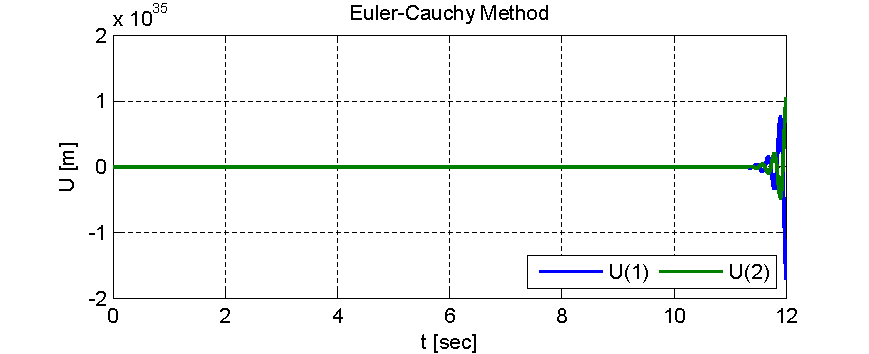
\includegraphics[width=\textwidth]{312_Euler.pdf}
\caption{A \ref{subsec:lingerj} gerjesztett rezgéses példa elmozdulásai Euler módszerrel.}
\label{fig:függlingerjeredm_euler}
\end{figure}
\begin{figure}[H]
\centering
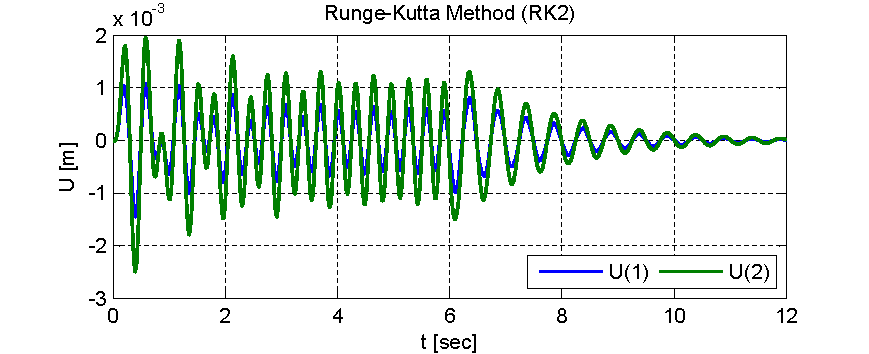
\includegraphics[width=\textwidth]{312_RK.pdf}
\caption{A \ref{subsec:lingerj} gerjesztett rezgéses példa elmozdulásai Runge-Kutta módszerrel.}
\label{fig:függlingerjeredm_rk}
\end{figure}
\begin{figure}[H]
\centering
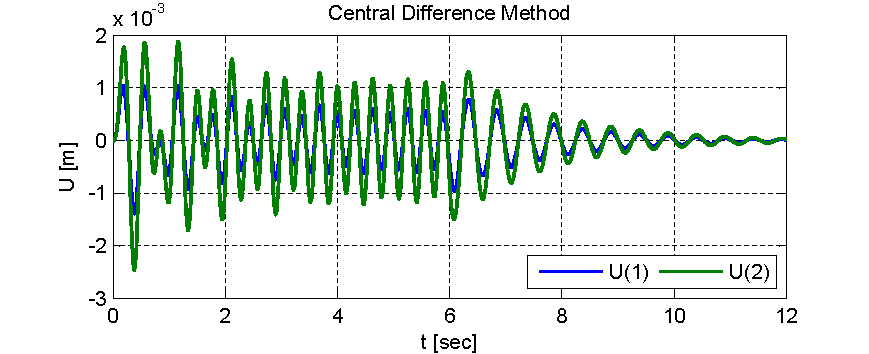
\includegraphics[width=\textwidth]{312_cendiff.pdf}
\caption{A \ref{subsec:lingerj} gerjesztett rezgéses példa elmozdulásai centrális differenciák módszerével.}
\label{fig:függlingerjeredm_centdiff}
\end{figure}

\begin{figure}[H]
\centering
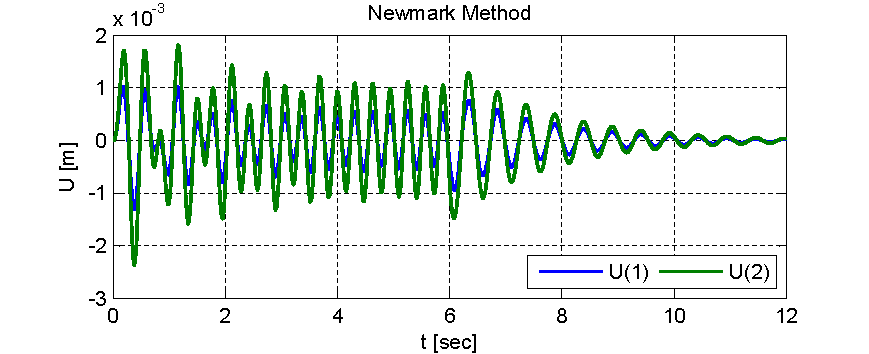
\includegraphics[width=\textwidth]{312_Newmark.pdf}
\caption{A \ref{subsec:lingerj} gerjesztett rezgéses példa elmozdulásai Newmark módszerrel.}
\label{fig:függlingerjeredm_newmark}
\end{figure}
\begin{figure}[H]
\centering
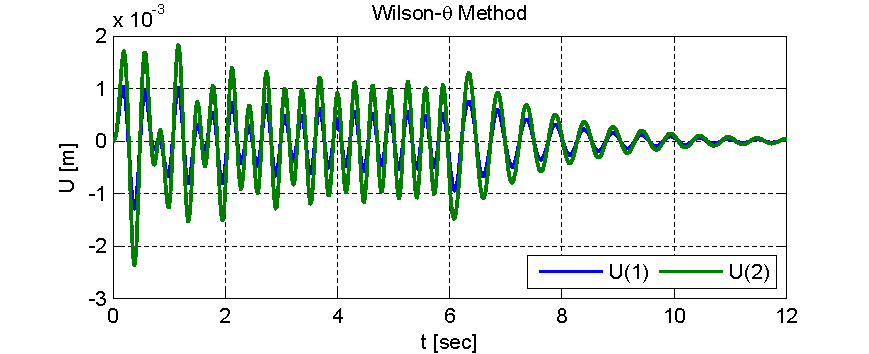
\includegraphics[width=\textwidth]{312_Wilson.pdf}
\caption{A \ref{subsec:lingerj} gerjesztett rezgéses példa elmozdulásai Wilson-$\boldsymbol\theta$ eljárással.}
\label{fig:függlingerjeredm_wilson}
\end{figure}
\begin{figure}[H]
\centering
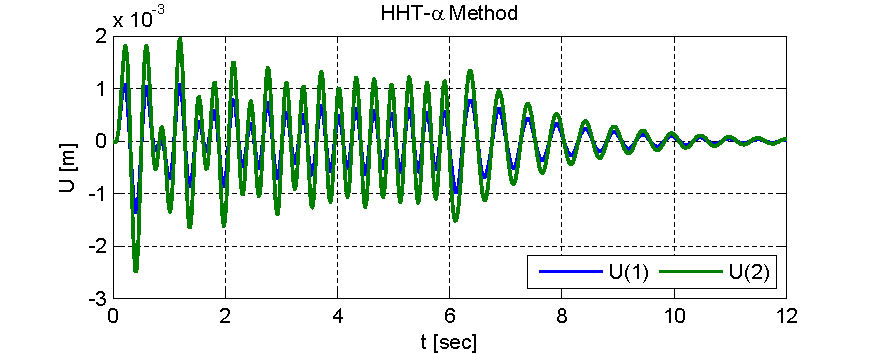
\includegraphics[width=\textwidth]{312_HHT.pdf}
\caption{A \ref{subsec:lingerj} gerjesztett rezgéses példa elmozdulásai HHT-$\alpha$ módszerrel.}
\label{fig:függlingerjeredm_hht}
\end{figure}
\begin{figure}[H]
\centering
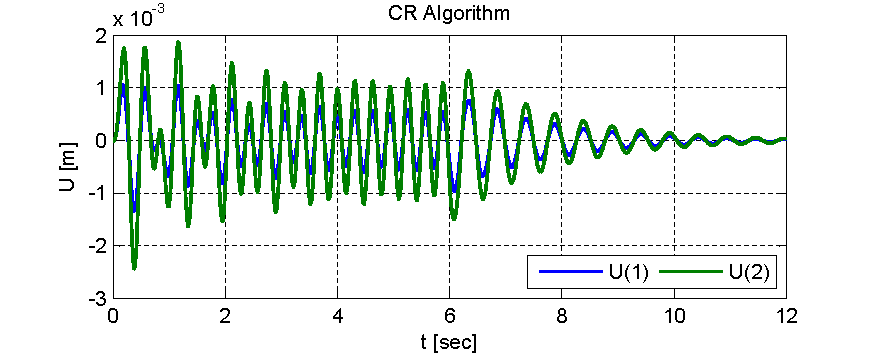
\includegraphics[width=\textwidth]{312_CR.pdf}
\caption{A \ref{subsec:lingerj} gerjesztett rezgéses példa elmozdulásai CR algoritmussal.}
\label{fig:függlingerjeredm_cr}
\end{figure}

\begin{figure}[H]
\centering
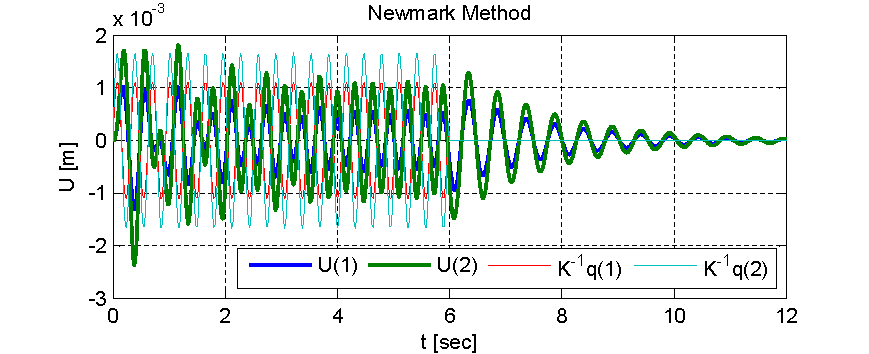
\includegraphics[width=\textwidth]{312_Newmark_Ku.pdf}
\caption{A \ref{subsec:lingerj} gerjesztett rezgéses példa elmozdulásai Newmark módszerrel és a statikus elmozdulás.}
\label{fig:függlingerjeredm_newmark_Ku}
\end{figure}


\section{A \ref{subsec:szabrezg} szabadrezgéses feladat eredményei}\label{sec:függ_szabrezg}

\subsection{A \ref{subsec:szabrezg} szabadrezgéses feladat elmozdulásai}\label{sec:függ_szabrezg_elm}

\begin{figure}[H]
\centering
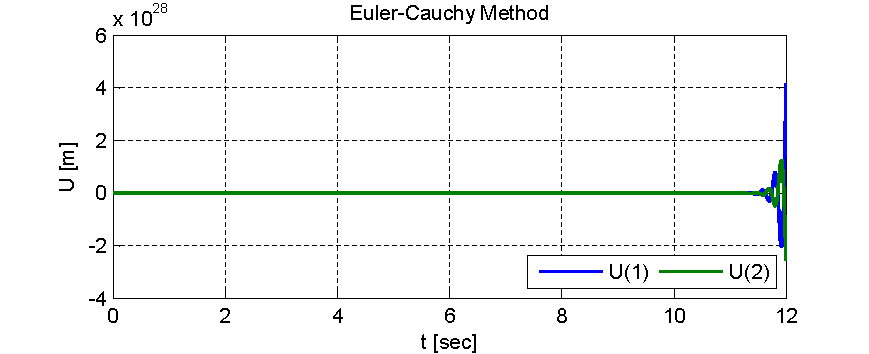
\includegraphics[width=\textwidth]{313_Euler.pdf}
\caption{A \ref{subsec:szabrezg} szabadrezgéses példa elmozdulásai Euler módszerrel.}
\label{fig:függszabrezg_er_euler}
\end{figure}

\begin{figure}[H]
\centering
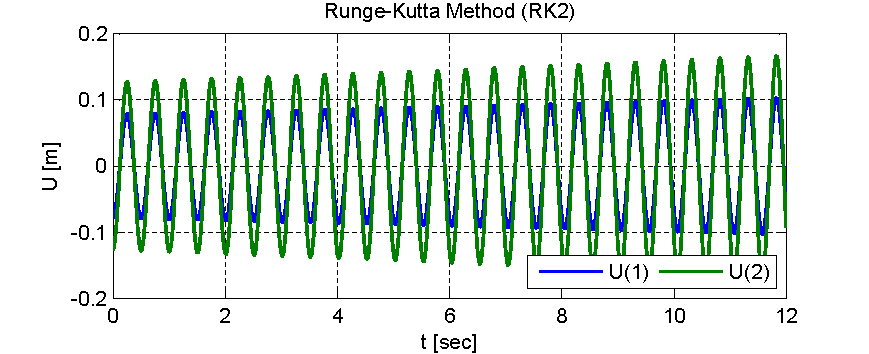
\includegraphics[width=\textwidth]{313_RK.pdf}
\caption{A \ref{subsec:szabrezg} szabadrezgéses példa elmozdulásai Runge-Kutta módszerrel.}
\label{fig:függszabrezg_er_rk}
\end{figure}

\begin{figure}[H]
\centering
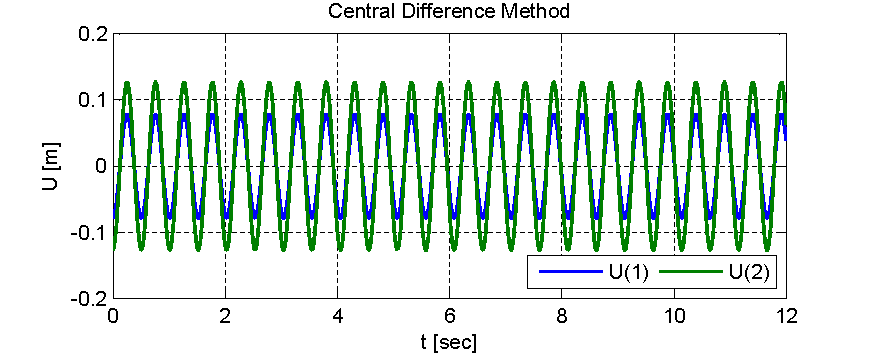
\includegraphics[width=\textwidth]{313_cendiff.pdf}
\caption{A \ref{subsec:szabrezg} szabadrezgéses példa elmozdulásai centrális differenciák módszerével.}
\label{fig:függszabrezg_er_centdiff}
\end{figure}

\begin{figure}[H]
\centering
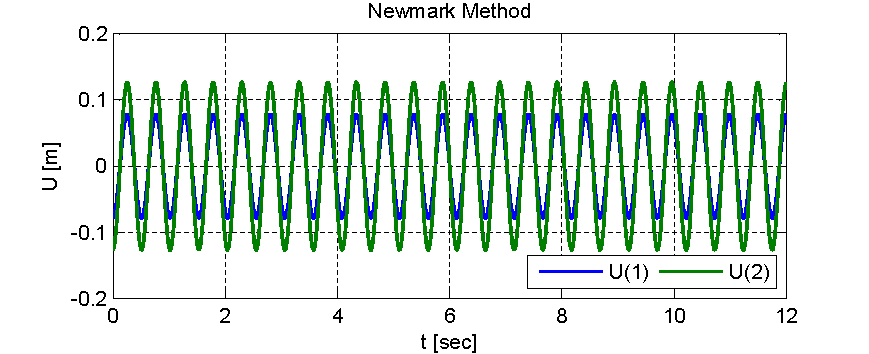
\includegraphics[width=\textwidth]{313_Newmark.pdf}
\caption{A \ref{subsec:szabrezg} gerjesztett rezgéses példa elmozdulásai Newmark módszerrel.}
\label{fig:függszabrezg_er_newmark}
\end{figure}

\begin{figure}[H]
\centering
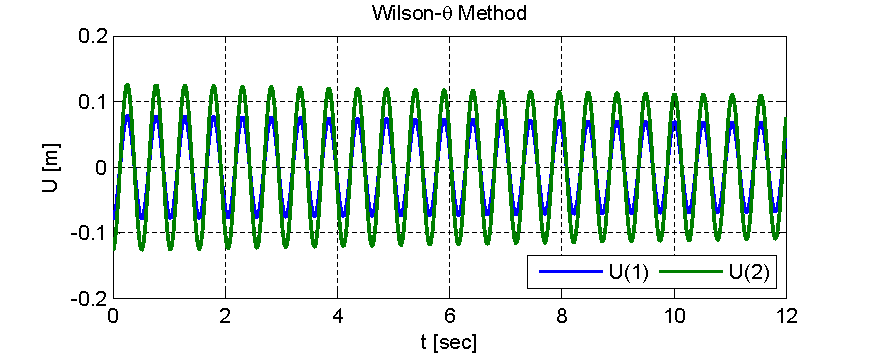
\includegraphics[width=\textwidth]{313_Wilson.pdf}
\caption{A \ref{subsec:szabrezg} szabadrezgéses példa elmozdulásai Wilson-$\boldsymbol\theta$ eljárással.}
\label{fig:függszabrezg_er_wilson}
\end{figure}

\begin{figure}[H]
\centering
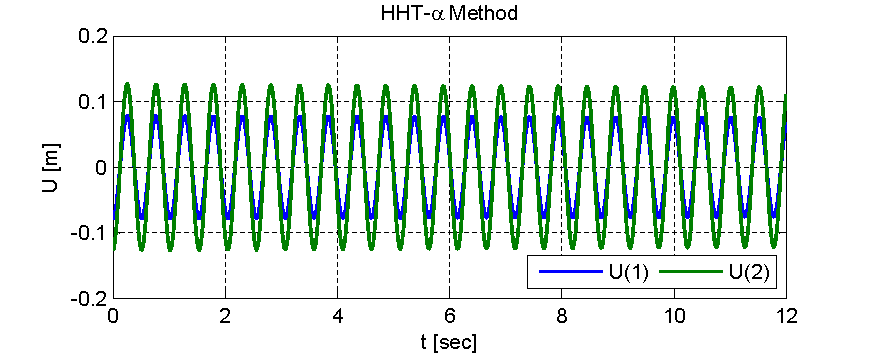
\includegraphics[width=\textwidth]{313_HHT.pdf}
\caption{A \ref{subsec:szabrezg} szabadrezgéses példa elmozdulásai HHT-$\alpha$ módszerrel.}
\label{fig:függszabrezg_er_hht}
\end{figure}

\begin{figure}[H]
\centering
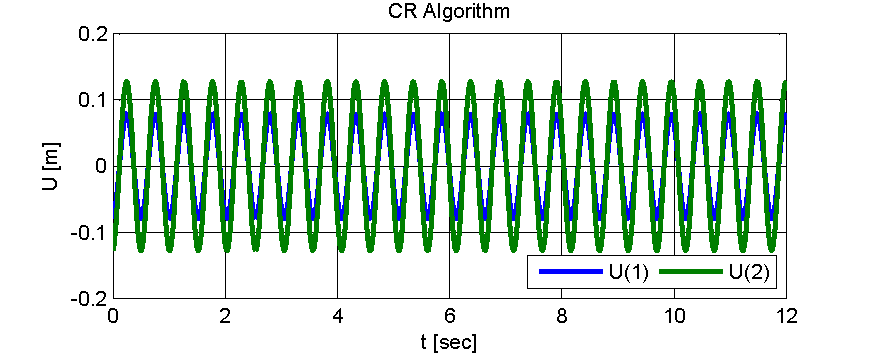
\includegraphics[width=\textwidth]{313_CR.pdf}
\caption{A \ref{subsec:szabrezg} szabadrezgéses példa elmozdulásai CR algoritmussal.}
\label{fig:függszabrezg_er_cr}
\end{figure}

\subsection{A \ref{subsec:szabrezg} szabadrezgéses feladat mechanikai energiái}\label{sec:függ_szabrezg_mechen}

\begin{figure}[H]
\centering
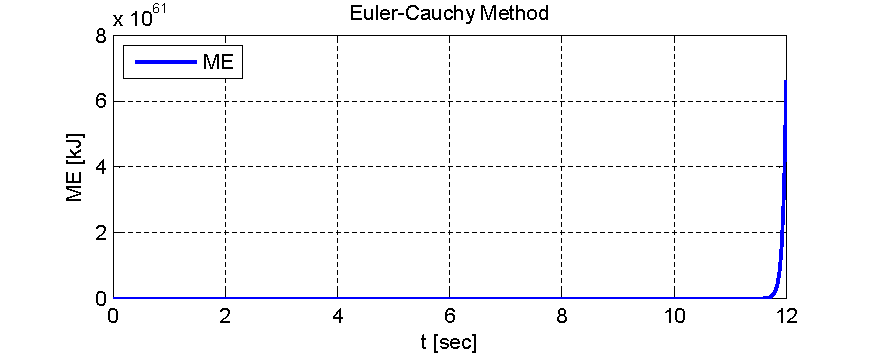
\includegraphics[width=\textwidth]{313_Euler_mechen.pdf}
\caption{A \ref{subsec:szabrezg} szabadrezgéses példa mechanikai energiája Euler módszerrel.}
% \label{fig:függszabrezg_er_mechen_euler}
\end{figure}

\begin{figure}[H]
\centering
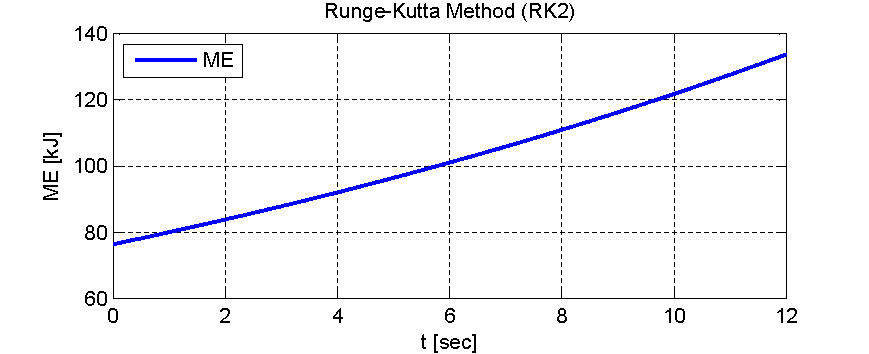
\includegraphics[width=\textwidth]{313_RK_mechen.pdf}
\caption{A \ref{subsec:szabrezg} szabadrezgéses példa mechanikai energiája Runge-Kutta módszerrel.}
% \label{fig:függszabrezg_er_mechen_rk}
\end{figure}

\begin{figure}[H]
\centering
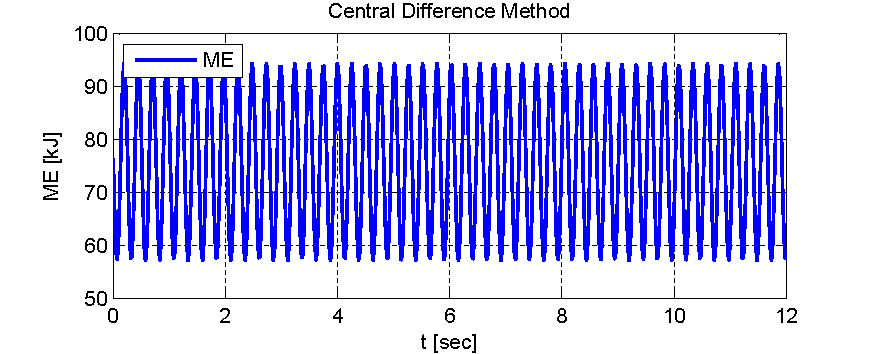
\includegraphics[width=\textwidth]{313_cendiff_mechen.pdf}
\caption{A \ref{subsec:szabrezg} szabadrezgéses példa mechanikai energiája centrális differenciák módszerével.}
% \label{fig:függszabrezg_er_mechen_centdiff}
\end{figure}

\begin{figure}[H]
\centering
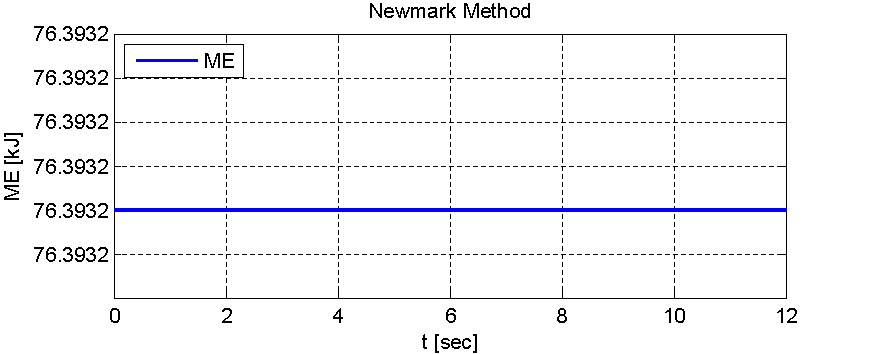
\includegraphics[width=\textwidth]{313_Newmark_mechen.pdf}
\caption{A \ref{subsec:szabrezg} szabadrezgéses példa mechanikai energiája Newmark módszerrel.}
% \label{fig:függszabrezg_er_mechen_newmark}
\end{figure}

\begin{figure}[H]
\centering
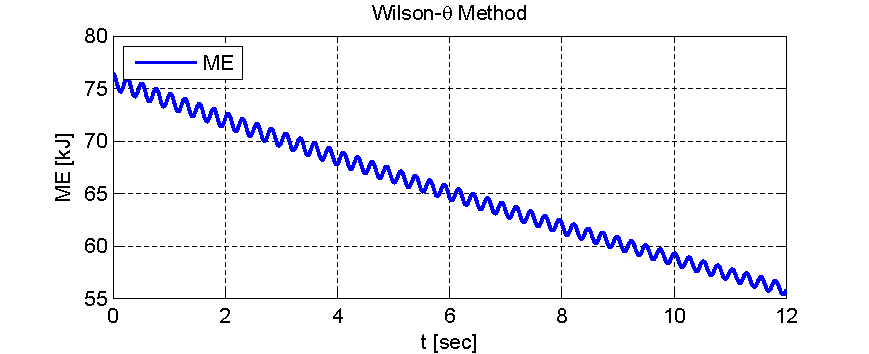
\includegraphics[width=\textwidth]{313_Wilson_mechen.pdf}
\caption{A \ref{subsec:szabrezg} szabadrezgéses példa mechanikai energiája Wilson-$\boldsymbol\theta$ eljárással.}
% \label{fig:függszabrezg_er_mechen_wilson}
\end{figure}

\begin{figure}[H]
\centering
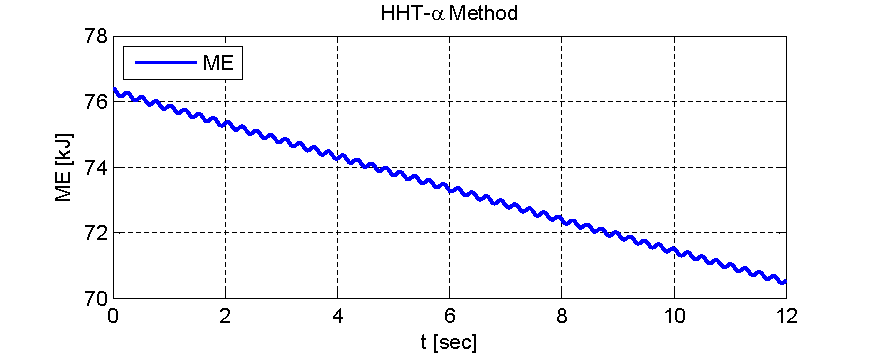
\includegraphics[width=\textwidth]{313_HHT_mechen.pdf}
\caption{A \ref{subsec:szabrezg} szabadrezgéses példa mechanikai energiája HHT-$\alpha$ módszerrel.}
% \label{fig:függszabrezg_er_mechen_hht}
\end{figure}

\begin{figure}[H]
\centering
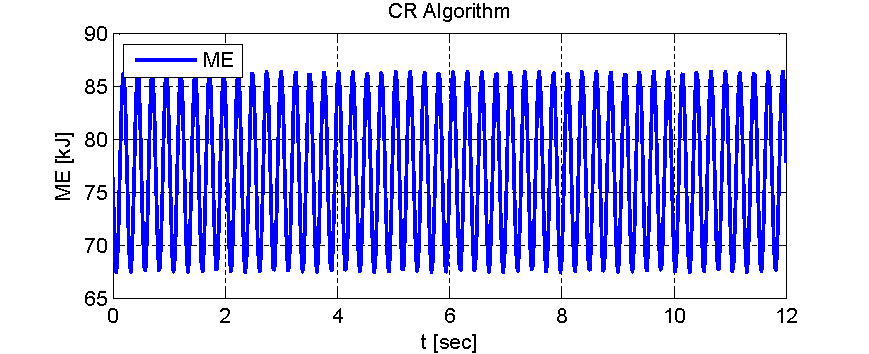
\includegraphics[width=\textwidth]{313_CR_mechen.pdf}
\caption{A \ref{subsec:szabrezg} szabadrezgéses példa mechanikai energiája CR algoritmussal.}
% \label{fig:függszabrezg_er_mechen_cr}
\end{figure}

\subsection{A \ref{subsec:szabrezg} szabadrezgéses feladat elmozdulásai fázistérben ábrázolva}\label{sec:függ_szabrezg_fázis}


\begin{figure}[H]
\centering
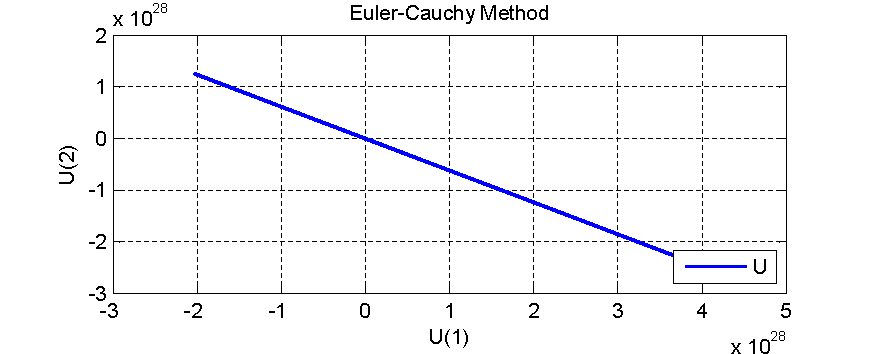
\includegraphics[width=\textwidth]{313_Euler_elm.pdf}
\caption{A \ref{subsec:szabrezg} szabadrezgéses példa elmozdulásai Euler módszerrel, fázistérben ábrázolva.}
% \label{fig:függszabrezg_er_elm_euler}
\end{figure}

\begin{figure}[H]
\centering
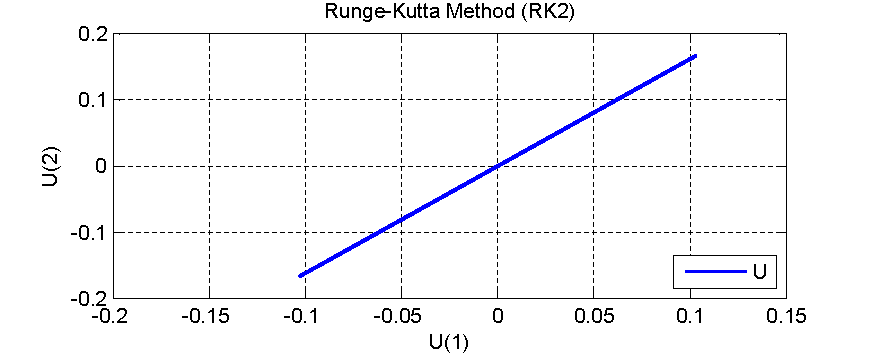
\includegraphics[width=\textwidth]{313_RK_elm.pdf}
\caption{A \ref{subsec:szabrezg} szabadrezgéses példa elmozdulásai Runge-Kutta módszerrel, fázistérben ábrázolva.}
% \label{fig:függszabrezg_er_elm_rk}
\end{figure}

\begin{figure}[H]
\centering
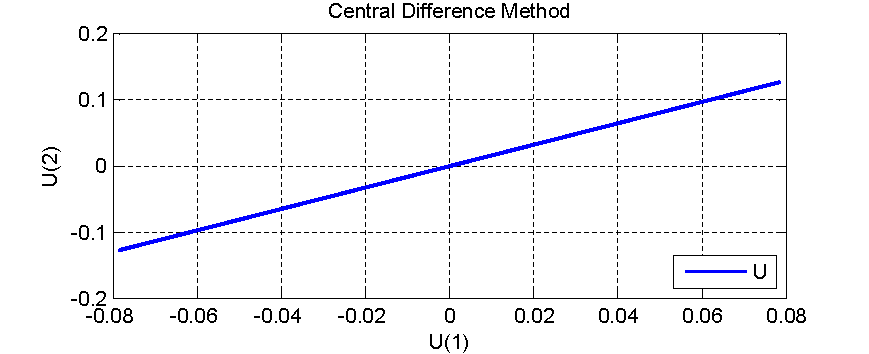
\includegraphics[width=\textwidth]{313_cendiff_elm.pdf}
\caption{A \ref{subsec:szabrezg} szabadrezgéses példa elmozdulásai centrális differenciák módszerével, fázistérben ábrázolva.}
% \label{fig:függszabrezg_er_elm_centdiff}
\end{figure}

\begin{figure}[H]
\centering
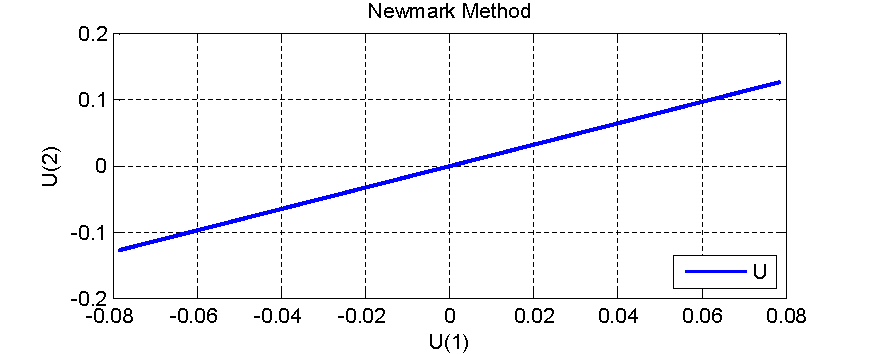
\includegraphics[width=\textwidth]{313_Newmark_elm.pdf}
\caption{A \ref{subsec:szabrezg} szabadrezgéses példa megoldása fázistérben ábrázolva Newmark módszerrel.}
% \label{fig:függszabrezg_er_elm_newmark}
\end{figure}

\begin{figure}[H]
\centering
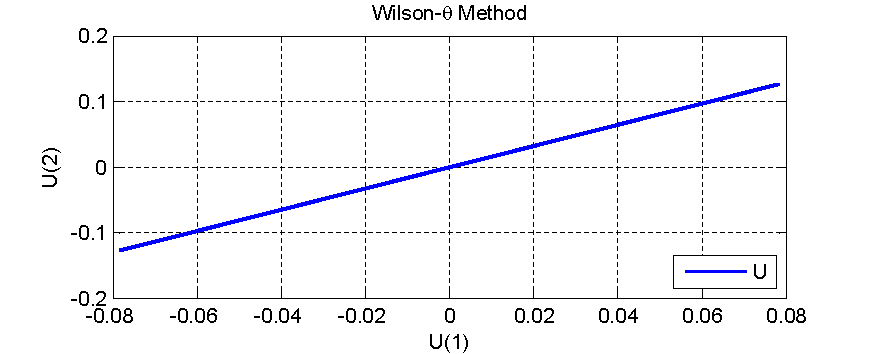
\includegraphics[width=\textwidth]{313_Wilson_elm.pdf}
\caption{A \ref{subsec:szabrezg} szabadrezgéses példa elmozdulásai Wilson-$\boldsymbol\theta$ eljárással, fázistérben ábrázolva.}
K\label{fig:függszabrezg_er_elm_wilson}
\end{figure}

\begin{figure}[H]
\centering
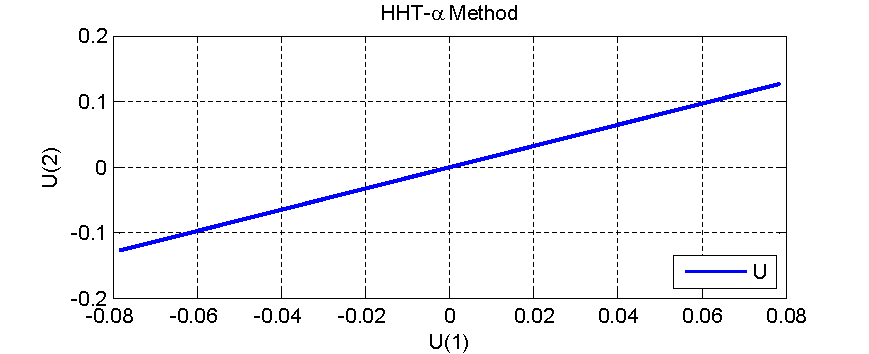
\includegraphics[width=\textwidth]{313_HHT_elm.pdf}
\caption{A \ref{subsec:szabrezg} szabadrezgéses példa elmozdulásai HHT-$\alpha$ módszerrel, fázistérben ábrázolva.}
% \label{fig:függszabrezg_er_elm_hht}
\end{figure}

\begin{figure}[H]
\centering
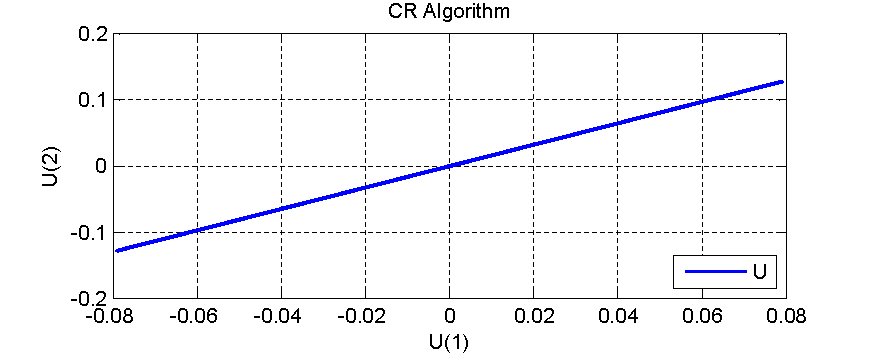
\includegraphics[width=\textwidth]{313_CR_elm.pdf}
\caption{A \ref{subsec:szabrezg} szabadrezgéses példa elmozdulásai CR algoritmussal, fázistérben ábrázolva.}
% \label{fig:függszabrezg_er_elm_cr}
\end{figure}

\section{A nemlineáris megoldó program eredményei}

\subsection{A \ref{subsec:nemlinstat} statikus vizsgálat eredményei}\label{sec:függ 322}


\begin{figure}[H]
\centering
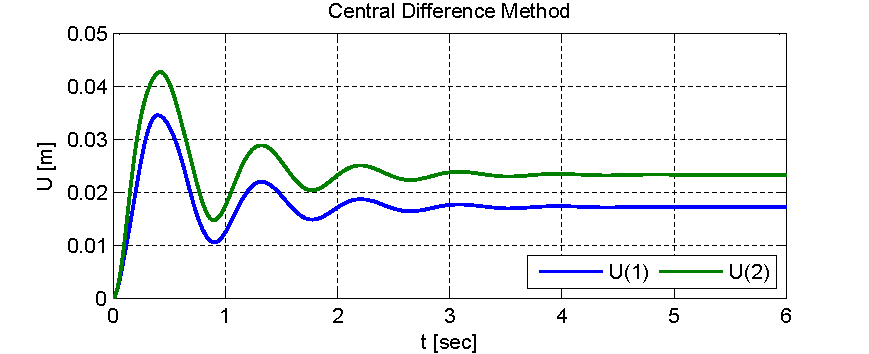
\includegraphics[width=\textwidth]{322_centdiff_kszi_0_1.pdf}
\caption{A \ref{subsec:nemlinstat} statikus probléma elmozdulásai centrális differenciák módszerével, $\xi = 0.1$-re.}
\label{fig:függ322_centdiff_0_1}
\end{figure}

\begin{figure}[H]
\centering
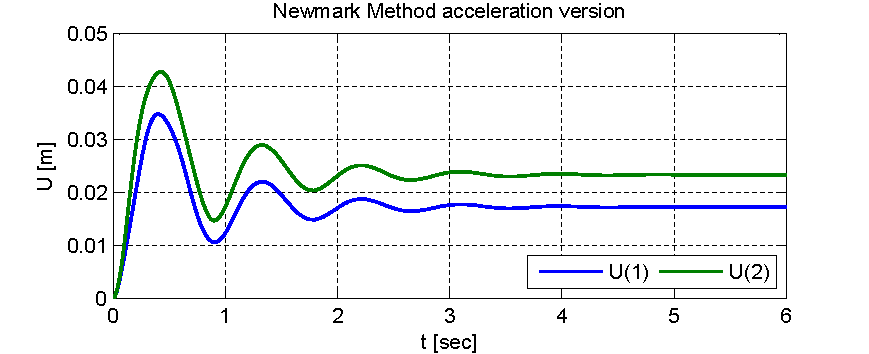
\includegraphics[width=\textwidth]{322_newmark_acc_kszi_0_1.pdf}
\caption{A \ref{subsec:nemlinstat} statikus probléma elmozdulásai a Newmark módszer gyorsulásos változatával, $\xi = 0.1$-re.}
\label{fig:függ322_newmark_acc_0_1}
\end{figure}

\begin{figure}[H]
\centering
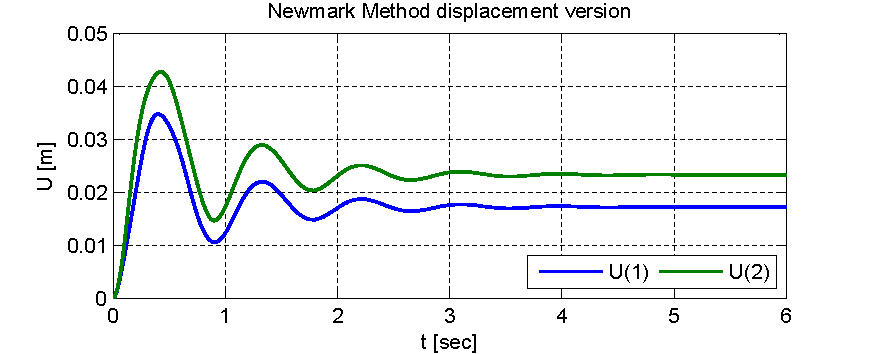
\includegraphics[width=\textwidth]{322_newmark_disp_kszi_0_1.pdf}
\caption{A \ref{subsec:nemlinstat} statikus probléma elmozdulásai a Newmark módszer elmozdulásos változatával, $\xi = 0.1$-re.}
\label{fig:függ322_newmark_disp_0_1}
\end{figure}

\begin{figure}[H]
\centering
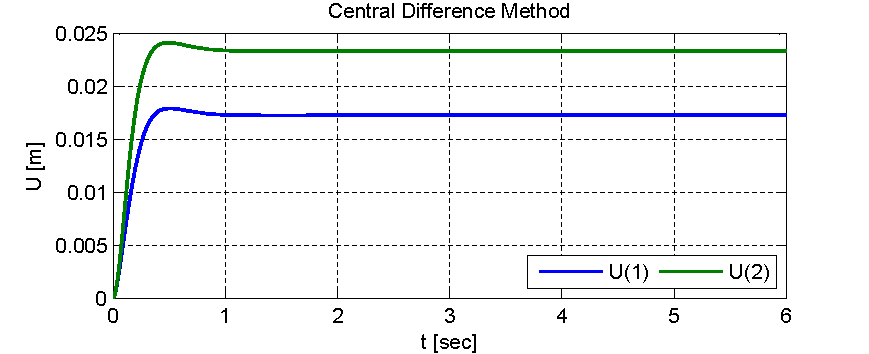
\includegraphics[width=\textwidth]{322_centdiff_kszi_0_5.pdf}
\caption{A \ref{subsec:nemlinstat} statikus probléma elmozdulásai centrális differenciák módszerével, $\xi = 0.5$-re.}
\label{fig:függ322_centdiff_0_5}
\end{figure}

\begin{figure}[H]
\centering
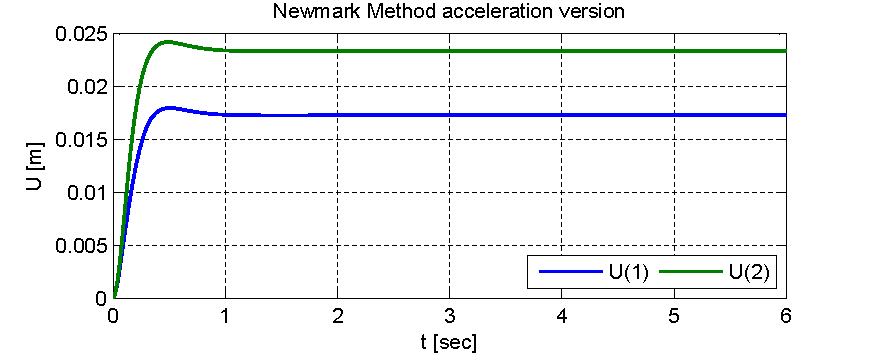
\includegraphics[width=\textwidth]{322_newmark_acc_kszi_0_5.pdf}
\caption{A \ref{subsec:nemlinstat} statikus probléma elmozdulásai a Newmark módszer gyorsulásos változatával, $\xi = 0.5$-re.}
\label{fig:függ322_newmark_acc_0_5}
\end{figure}

\begin{figure}[H]
\centering
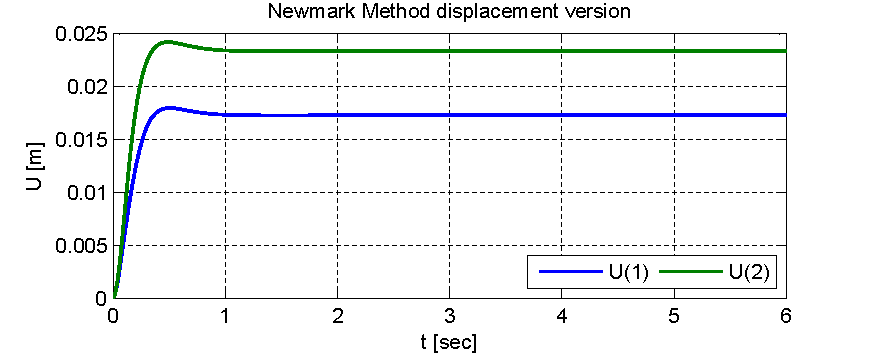
\includegraphics[width=\textwidth]{322_newmark_disp_kszi_0_5.pdf}
\caption{A \ref{subsec:nemlinstat} statikus probléma elmozdulásai a Newmark módszer elmozdulásos változatával, $\xi = 0.5$-re.}
\label{fig:függ322_newmark_disp_0_5}
\end{figure}

\begin{figure}[H]
\centering
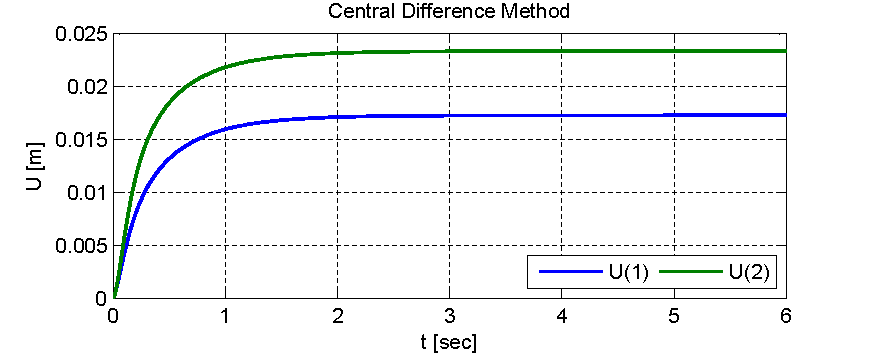
\includegraphics[width=\textwidth]{322_centdiff_kszi_1_1.pdf}
\caption{A \ref{subsec:nemlinstat} statikus probléma elmozdulásai centrális differenciák módszerével, $\xi = 1.1$-re.}
\label{fig:függ322_centdiff_1_1}
\end{figure}

\begin{figure}[H]
\centering
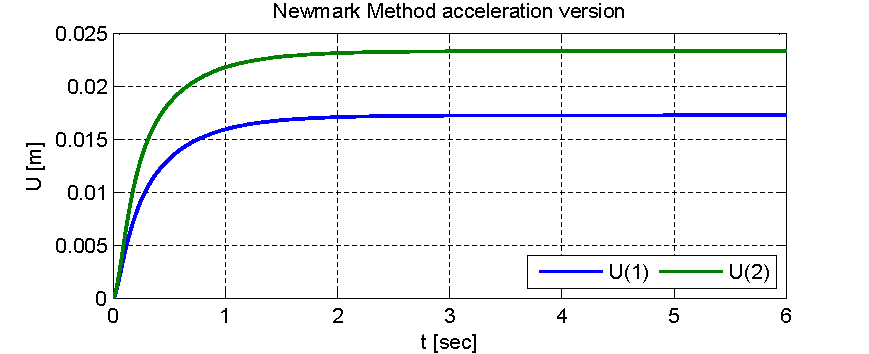
\includegraphics[width=\textwidth]{322_newmark_acc_kszi_1_1.pdf}
\caption{A \ref{subsec:nemlinstat} statikus probléma elmozdulásai a Newmark módszer gyorsulásos változatával, $\xi = 1.1$-re.}
\label{fig:függ322_newmark_acc_1_1}
\end{figure}

\begin{figure}[H]
\centering
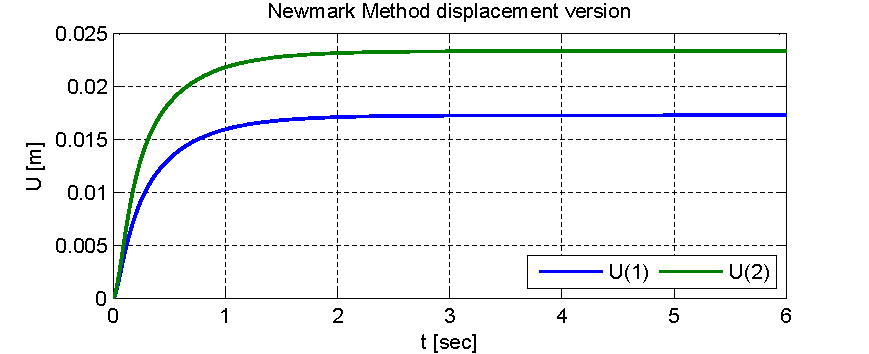
\includegraphics[width=\textwidth]{322_newmark_disp_kszi_1_1.pdf}
\caption{A \ref{subsec:nemlinstat} statikus probléma elmozdulásai a Newmark módszer elmozdulásos változatával, $\xi = 1.1$-re.}
\label{fig:függ322_newmark_disp_1_1}
\end{figure}


\subsection{A \ref{subsec:nemlindin} dinamikus vizsgálat eredményei}\label{sec:függ 323}


\begin{figure}[H]
\centering
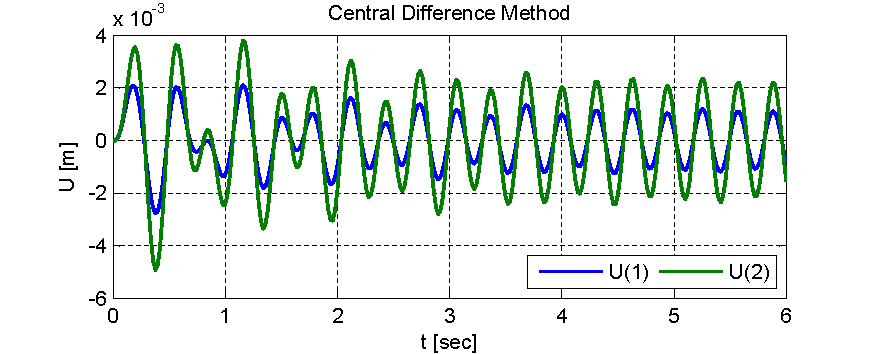
\includegraphics[width=\textwidth]{323_centdiff.pdf}
\caption{A \ref{subsec:nemlindin} dinamikus probléma elmozdulásai centrális differenciák módszerével.}
\label{fig:függ323_centdiff}
\end{figure}

\begin{figure}[H]
\centering
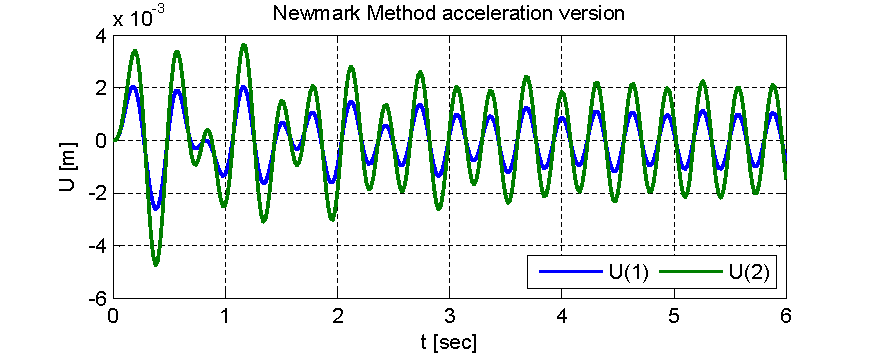
\includegraphics[width=\textwidth]{323_Newmark_acc.pdf}
\caption{A \ref{subsec:nemlindin} dinamikus probléma elmozdulásai a Newmark módszer gyorsulásos változatával.}
\label{fig:függ323_newmark_acc}
\end{figure}

\begin{figure}[H]
\centering
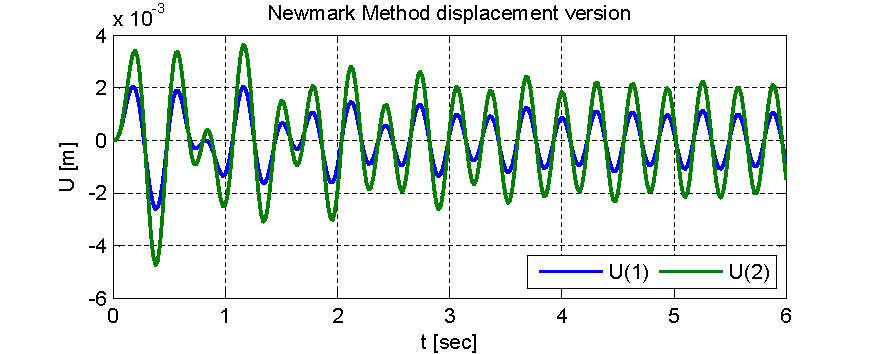
\includegraphics[width=\textwidth]{323_Newmark_disp.pdf}
\caption{A \ref{subsec:nemlindin} dinamikus probléma elmozdulásai a Newmark módszer elmozdulásos változatával.}
\label{fig:függ323_newmark_disp}
\end{figure}


\begin{figure}[H]
\centering
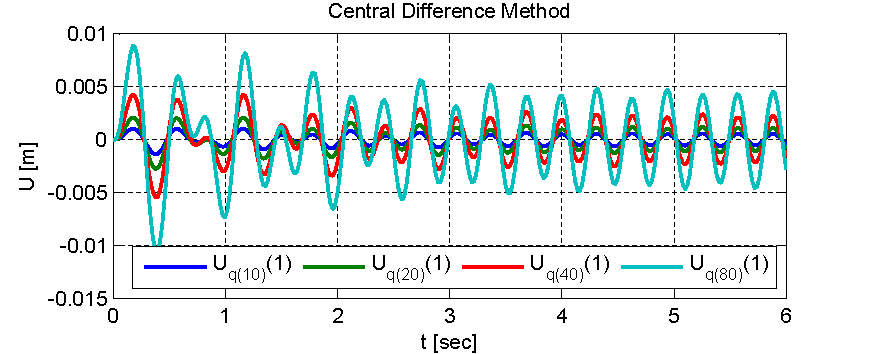
\includegraphics[width=\textwidth]{323_centdiff_q_var.pdf}
\caption{A \ref{subsec:nemlindin} dinamikus probléma megoldásai az első csomópontra  centrális differenciák módszerével különböző terhelésekre.}
\label{fig:függ323_newmark_disp_q_var_1}
\end{figure}

\begin{figure}[H]
\centering
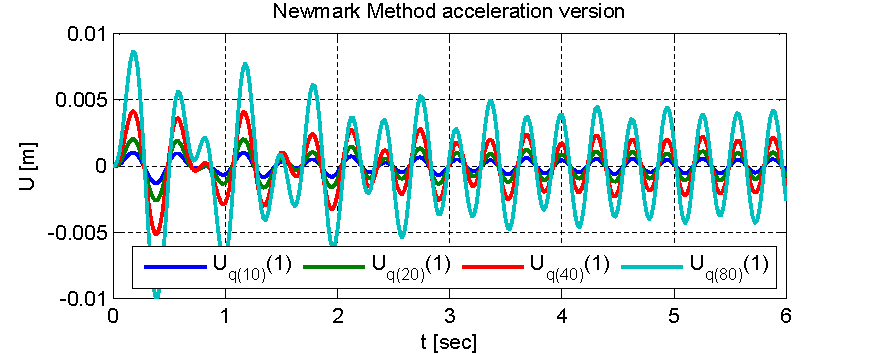
\includegraphics[width=\textwidth]{323_Newmark_acc_q_var.pdf}
\caption{A \ref{subsec:nemlindin} dinamikus probléma megoldásai az első csomópontra a Newmark módszer gyorsulásos változatával különböző terhelésekre.}
\label{fig:függ323_newmark_disp_q_var_1}
\end{figure}

\begin{figure}[H]
\centering
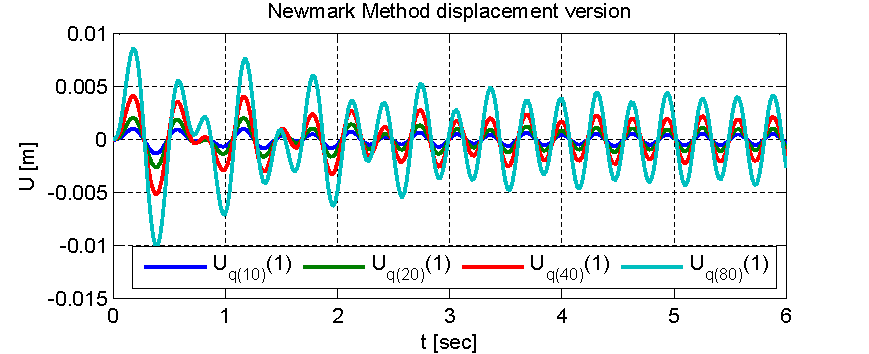
\includegraphics[width=\textwidth]{323_Newmark_disp_q_var.pdf}
\caption{A \ref{subsec:nemlindin} dinamikus probléma megoldásai az első csomópontra a Newmark módszer elmozdulásos változatával különböző terhelésekre.}
\label{fig:függ323_newmark_disp_q_var_1}
\end{figure}



\chapter{A hibrid szimulációs program kódja}\label{chap: függ hibrid prog}

\lstinputlisting{"MATLAB/hibrid/main.m"}
 \lstinputlisting{"MATLAB/hibrid_72/init_system.m"}
 \lstinputlisting{"MATLAB/hibrid/init_conditions.m"}

 \lstinputlisting{"MATLAB/hibrid/convert_num2lab.m"}
 \lstinputlisting{"MATLAB/hibrid/labor.m"}
 \lstinputlisting{"MATLAB/hibrid/convert_lab2num.m"}
 \lstinputlisting{"MATLAB/hibrid/timestep.m"}
 \lstinputlisting{"MATLAB/hibrid/resisting_force.m"}
 \lstinputlisting{"MATLAB/hibrid/U_num2lab.m"}
 \lstinputlisting{"MATLAB/hibrid/f_s_lab2num.m"}
 
 Az  földrengések adatait beolvasó függvény:
 \lstinputlisting{"MATLAB/hibrid_72/EQ_load.m"}

 